\documentclass[12pt]{article}

\usepackage{lmodern}
\usepackage[utf8]{inputenc}
\usepackage[T1]{fontenc}
\usepackage[french]{babel}
\usepackage{url}
\usepackage{graphicx}
\graphicspath{ {./img/} }

\title{\textbf{Analyse de données d’eye-tracking en Réalité Virtuelle}}
\author{\Large{Adonis Stavridis}}
\date{Février 2021}

\begin{document}

% ----------------------------------------------------------------------------
% TITLEPAGE
% ----------------------------------------------------------------------------

\maketitle
\tableofcontents
\pagebreak

% ----------------------------------------------------------------------------
% INTRODUCTION
% ----------------------------------------------------------------------------

\section{Introduction}
L'eye-tracking \cite{wiki:eye_tracking}, ou oculométrie, est une technologie
assez récente qui détermine la position du regard d'un individu. Des capteurs
spéciaux envoient des rayons infrarouges vers les yeux d'un individu et ceux-ci
sont réfléchis, leur permettant ainsi de déterminer ses mouvements oculaires
sur un écran. Elle établie alors une nouvelle interface entre Homme et machine
et est devenue aujourd'hui une technologie principale dans des études liées au
système visuel humain, à la psychologie, au marketing et design. Elle est en
fait dèjà très utilisée dans les jeux vidéos. Un domaine où cette technologie
reste encore peu developpée est la réalité virtuelle.

\bigskip
Déterminer la position du regard d'un individu sur un écran permet d'effectuer
des études quantitatives et qualitatives sur de multiples supports, et ainsi
comprendre les comportements humains dans différentes situations. L'eye-tracking
s'avère donc être très pratique pour étudier sur un document par exemple, les
zones qui sont le plus attrayantes et celles qui le sont moins. Cependant,
certaines études ont besoin d'un environment plus réalistes. La réalité
virtuelle ajoute une nouvelle couche d'immersion, permettant à un individu de
se sentir et agir de façon plus réaliste. Ainsi, la réalité virtuelle
permettrait de livrer des résultats beaucoup plus fiables pour certains
domaines, et ainsi aider à l'avancement des recherches sur le comportement
humain.

% ----------------------------------------------------------------------------
% MATERIEL
% ----------------------------------------------------------------------------

\section{Capteurs d'oculométrie}

Pour l'instant, les meilleurs produits liés à l'eye-tracking sont ceux crées
par l'entreprise Tobii \cite{tobii} et HTC Vive \cite{htc_vive_pro_eye}. Elles
proposent des solutions dans plusieurs domaines, des capteurs simples pouvant
être utilisés pour suivre les mouvements sur un écran, des solutions plus
professionnelles pour effectuer des captures dans le monde réel, mais aussi des
produits pour des individus qui nécessitent de l'assistance.

\bigskip
Le capteur le plus basique est une barre à placer en dessous ou au dessus d'un
écran, qui va donc capturer les mouvements oculaires d'un individu et déterminer
la position de son regard sur cet écran. Ce capteur permet d'enregistrer toutes
les données afin de les étudier et effectuer des analyses statistiques. C'est un
produit très pratique, mais laisse peu de liberté de mouvement. Des nouveaux
capteurs d'oculométrie ont éte intégrés à des casques de réalité virtuelle,
pour profiter du mouvement libre dans un monde tri-dimensionnel.

\begin{figure}[htpb]
  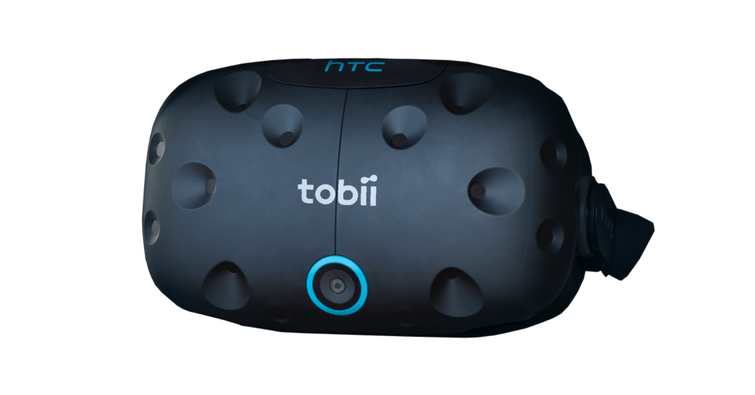
\includegraphics[width=\textwidth,keepaspectratio=true]{tobiivr.png}
  \caption{Casque de réalité virtuelle Tobii VR}
\end{figure}

L'ajout de l'eye-tracking dans la réalité virtuelle permet essentielment de
faire du rendu fovéal \cite{wiki:foveated_rendering} : les yeux ne se
focalisent qu'en une seule région tandis que le reste du champ visuel est flou.
Cette méthode de rendu propose d'effectuer un rendu de très haute qualité à la
région de focalisation mais une qualité de rendu moins important dans les reste
du champ périphérique. La réalité virtuelle a souvent besoin de beaucoup de
puissance de calcul, et donc cette technique de rendu associée avec
l'eye-tracking permettrait de faire des gains en puissance de calcul mais aussi
en qualité de rendu, en plus des fonctionnalités de tout capteur basique.

% ----------------------------------------------------------------------------
% LOGICIELS
% ----------------------------------------------------------------------------

\section{Logiciels}

De nos jours, la plupart des gens possédent un appareil électronique avec une
caméra intergrée, que ce soit une webcam ou la caméra d'un smartphone. Il n'est
pas nécessaire d'acheter du matériel professionnel pour profiter de la
technologie d'eye-tracking. Il existe plusieurs logiciels et bibliothèques qui
permettent d'effectuer de l'oculométrie, facilement et gratuitement aussi.

\subsection{OpenCV}

L'une des bibliothèques les plus utilisées dans le traitement d'images en temps
réel et en vision par ordinateur ou Computer Vision est OpenCV \cite{opencv}.
Elle propose des fonctionnalités pour traiter des données brutes d'images, mais
aussi une grande variété d'outils issus de l'état de l'art en vision des
ordinateurs (détection de visage par exemple) et des algorithmes d'apprentissage
artificiel. En tout, c'est une bibliothèque très compléte, pour la majorité des
domaines de la vision par ordinateur, mais pas forcément spécialisée dans
l'oculométrie. Il est possible toutefois d'écrire des algorithmes pour suivre
le regard grace aux outils mis à disposition par la bibliothèque. Il existe
également de jeux de données assez grands mis à disposition en ligne, tel que
NVGaze \cite{nvgaze} de NVidia, pour entrainer des réseaux de neurones à
éstimer le regard grace à des images \cite{gaze_tracking}. OpenCV propose plein
d'outils de visualisation des données en temps réel, mais aucun pour leur
exploitation.

\bigskip
Le grand avantage de OpenCV est son age et popularité. Elle est la bibliothèque
de référence dans le domaine de la vision par ordinateur, propose parmi des
outils très optimisés, tout en restant bien documenté. C'est aussi un projet
open-source, et c'est pour cela qu'elle rassemble une grande communauté.
Puisqu'elle n'est pas spécialisée dans l'eye-tracking, elle ne propose pas
d'outils d'analyse et de visualisation de données, nécessaires en oculométrie.

\subsection{PyGaze}

Une autre bibliothèque très intéressante est PyGaze \cite{pygaze}. C'est une
toolbox permettant de suivre le regard sur un écran grace à une caméra ou
webcam. Elle propose également des outils pour analyser les données
enregistrées, lors d'une séance d'eye-tracking. Ces outils permettent de créer
plusieurs types d'images pour suivre le regard au fur et à mesure du temps.
Parmi ces images se trouvent des cartes de fixations, des heatmap et des schémas
du chemin du regard. Elle permettent de facilement comprendre les données et
d'en tirer des conclusions plus rapidement. En plus, la bibliothèque PyGaze peut
être utilisée avec la SDK de Tobii pour profiter de toutes les fonctionnalités
des produits Tobii.

\bigskip
Cette bibliothèque est donc idéale pour visualiser les données récupérées grace
àl'oculométrie, de façon simple et efficace. Cette libraire est assez bien
documentée aussi. PyGaze est donc vraiment intéressante à utiliser, en
combinaison avec les capteurs Tobii pour tirer profit d'un maximum de données
et créer des images de synthése les plus concluantes possibles. Ces-dernieres
sont très importantes pour permettre de tirer les bonnes conclusions.

\begin{figure}[htpb]
  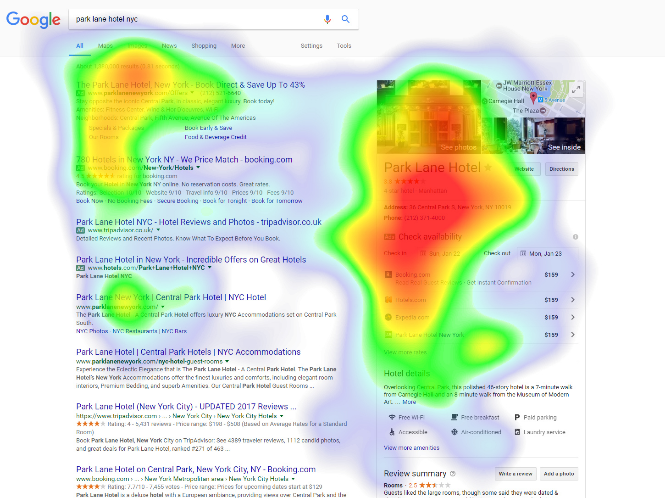
\includegraphics[width=\textwidth,keepaspectratio=true]{heatmap.png}
  \caption{Exemple de heatmap sur une page de recherche sur Google}
\end{figure}

\subsection{GazeParser}



\begin{itemize}
  \item NVGaze
  \item https://imotions.com/blog/10-terms-metrics-eye-tracking/
\end{itemize}

% ----------------------------------------------------------------------------
% CONCLUSION
% ----------------------------------------------------------------------------

\section{Conclusion}

% ----------------------------------------------------------------------------
% BIBLIOGRAPHIE
% ----------------------------------------------------------------------------

\pagebreak
\bibliographystyle{unsrt}
\bibliography{recherches}

\end{document}
